% Created with jtex v.1.0.20
\documentclass[twocolumn, switch]{article}
\usepackage{preprint}
\usepackage{hyperref}
\usepackage[numbers,square]{natbib}

%%%%%%%%%%%%%%%%%%%%%%%%%%%%%%%%%%%%%%%%%%%%%%%%%%
%%%%%%%%%%%%%%%%%%%%  imports  %%%%%%%%%%%%%%%%%%%
\usepackage{amsmath}
\usepackage{graphicx}
%%%%%%%%%%%%%%%%%  math commands  %%%%%%%%%%%%%%%%
\newcommand{\CRRA}{\rho}
\newcommand{\cNrm}{c}
\newcommand{\uFunc}{\mathbf{u}}
\newcommand{\Ex}{\mathbf{\mathbb{E}}}
\newcommand{\DiscFac}{\beta}
\newcommand{\cLvl}{\mathbf{c}}
\newcommand{\Rfree}{\text{R}}
\newcommand{\PermGroShk}{\mathcal{G}}
\newcommand{\tranShk}{\xi}
\newcommand{\aLvl}{\mathbf{a}}
\newcommand{\mLvl}{\mathbf{m}}
\newcommand{\pLvl}{\mathbf{p}}
\newcommand{\yLvl}{\mathbf{y}}
\newcommand{\rfree}{\text{r}}
\newcommand{\PermGroFac}{G}
\newcommand{\permShk}{\psi}
\newcommand{\tranShkEmp}{\theta}
\newcommand{\WorstProb}{\wp}
\newcommand{\permShkMin}{\underline{\permShk}}
\newcommand{\permShkMax}{\bar{\permShk}}
\newcommand{\tranShkEmpMin}{\underline{\tranShkEmp}}
\newcommand{\tranShkEmpMax}{\bar{\tranShkEmp}}
\newcommand{\mNrm}{m}
\newcommand{\RNrmByG}{\mathcal{R}}
\newcommand{\aNrm}{a}
\newcommand{\vFunc}{\mathbf{v}}
\newcommand{\uPrime}{\uFunc'}
\newcommand{\AbsPatFac}{\Phi}
\newcommand{\cFunc}{\mathbf{c}}
\newcommand{\cFuncOpt}{\bar{\cFunc}}
\newcommand{\cFuncApprox}{\grave{\cFunc}}
\newcommand{\hNrm}{h}
\newcommand{\hNrmOpt}{\bar{\hNrm}}
\newcommand{\MPC}{\boldsymbol{\kappa}}
\newcommand{\MPCmin}{\underline{\MPC}}
\newcommand{\hNrmPes}{\underline{\hNrm}}
\newcommand{\tranShkMin}{\underline{\tranShk}}
\newcommand{\mNrmMin}{\underline{\mNrm}}
\newcommand{\mNrmEx}{\ddot{\mNrm}}
\newcommand{\hNrmEx}{\ddot{\hNrm}}
\newcommand{\cFuncPes}{\underline{\cFunc}}
\newcommand{\cFuncReal}{\hat{\cFunc}}
\newcommand{\modRte}{\boldsymbol{\bar{\omega}}}
\newcommand{\logmNrmEx}{\boldsymbol{\mu}}
\newcommand{\logitModRte}{\boldsymbol{\chi}}
\newcommand{\logitModRteFunc}{\bar{\logitModRte}}
\newcommand{\logitModRteFuncApprox}{\grave{\logitModRteFunc}}
\newcommand{\PDV}{\operatorname{PDV}}
\newcommand{\PDVCoverc}{\mathcal{C}}
\newcommand{\vFuncOpt}{\bar{\vFunc}}
\newcommand{\vInv}{{\scriptsize \boldsymbol{\Lambda}}}
\newcommand{\vInvOpt}{\bar{\vInv}}
\newcommand{\vFuncReal}{\hat{\vFunc}}
\newcommand{\vInvReal}{\hat{\vInv}}
\newcommand{\valModRte}{\boldsymbol{\Omega}}
\newcommand{\valModRteReal}{\hat{\valModRte}}
\newcommand{\logitValModRte}{\boldsymbol{X}}
\newcommand{\logitValModRteReal}{\hat{\logitValModRte}}
\newcommand{\MPCmax}{\bar{\MPC}}
\newcommand{\mNrmCusp}{\mNrm^*}
\newcommand{\mNrmCuspEx}{\ddot{\mNrm}^*}
\newcommand{\modRtePes}{\boldsymbol{\underline{\omega}}}
\newcommand{\cFuncLoTightUpBd}{\grave{\check{\cFunc}}}
\newcommand{\mNrmLoTightUpBd}{\grave{\check{\mNrm}}}
\newcommand{\mNrmHiTightUpBd}{\grave{\hat{\mNrm}}}
\newcommand{\cFuncMidTightUpBd}{\grave{\tilde{\cFunc}}}
\newcommand{\cFuncHiTightUpBd}{\grave{\hat{\cFunc}}}
\newcommand{\wFuncCont}{\mathbf{w}}
\newcommand{\logitValModRteApprox}{\grave{\logitValModRte}}
\newcommand{\valModRteApprox}{\grave{\valModRte}}
\newcommand{\modRteMu}{\modRte^{\logmNrmEx}}
\newcommand{\logitModRteMu}{\logitModRte^{\logmNrmEx}}
\newcommand{\vInvOptDeriv}{\vInvOpt^{\mNrm}}
\newcommand{\vInvRealDeriv}{\vInvReal^{\mNrm}}
\newcommand{\valModRteRealDerivmu}{\valModRteReal^{\logmNrmEx}}
\newcommand{\logitValModRteRealDerivmu}{\logitValModRteReal^{\logmNrmEx}}
\newcommand{\vFuncRealDeriv}{\vFuncReal^{\mNrm}}
\newcommand{\uDoublePrime}{\uFunc''}
\newcommand{\vFuncRealDerivSecond}{\vFuncReal^{\mNrm\mNrm}}
\newcommand{\vInvRealDerivSecond}{\vInvReal^{\mNrm\mNrm}}
\newcommand{\Risky}{\mathbf{R}}
\newcommand{\Nrml}{\mathcal{N}}
\newcommand{\std}{\sigma}
\newcommand{\risky}{\mathbf{r}}
%%%%%%%%%%%%%%%%%%%%%%%%%%%%%%%%%%%%%%%%%%%%%%%%%%


% colors for hyperlinks
\hypersetup{colorlinks=true, linkcolor=purple, urlcolor=blue, citecolor=cyan, anchorcolor=black}

\usepackage[utf8]{inputenc}	% allow utf-8 input
\usepackage[T1]{fontenc}
\usepackage{xcolor}
\usepackage{lineno}					% Line numbers
\usepackage{tikz} 					% ORCiD insertion

%% Bibliography options
\bibliographystyle{unsrtnat}

 %% Special figure caption options
\usepackage{newfloat}
\DeclareFloatingEnvironment[name={Supplementary Figure}]{suppfigure}
\usepackage{sidecap}
\sidecaptionvpos{figure}{c}

% Section title spacing  options
\usepackage{titlesec}
\titlespacing\section{0pt}{12pt plus 3pt minus 3pt}{1pt plus 1pt minus 1pt}
\titlespacing\subsection{0pt}{10pt plus 3pt minus 3pt}{1pt plus 1pt minus 1pt}
\titlespacing\subsubsection{0pt}{8pt plus 3pt minus 3pt}{1pt plus 1pt minus 1pt}

\definecolor{lime}{HTML}{A6CE39}
\DeclareRobustCommand{\orcidicon}{
	
\begin{tikzpicture}
	\draw[lime, fill=lime] (0,0)
	circle [radius=0.16]
	node[white] {{\fontfamily{qag}\selectfont \tiny ID}};
	\draw[white, fill=white] (-0.0625,0.095)
	circle [radius=0.007];
	\end{tikzpicture}
	\hspace{-2mm}
}

%%%%%%%%%%%%%%%%   Title   %%%%%%%%%%%%%%%%
\title{The Method of Moderation}

% Add watermark with submission status
% Awaiting watermark support
% \usepackage{xwatermark}
% % Left watermark
% \newwatermark[firstpage,color=gray!60,angle=90,scale=0.32, xpos=-4.05in,ypos=0]{\href{https://doi.org/}{\color{gray}{Publication doi}}}
% % Right watermark
% \newwatermark[firstpage,color=gray!60,angle=90,scale=0.32, xpos=3.9in,ypos=0]{\href{https://doi.org/}{\color{gray}{Preprint doi}}}
% % Bottom watermark
% \newwatermark[firstpage,color=gray!90,angle=0,scale=0.28, xpos=0in,ypos=-5in]{*correspondence: \texttt{}}

%%%%%%%%%%%%%%%  Author list  %%%%%%%%%%%%%%%
\usepackage{authblk}
\renewcommand*{\Authfont}{\bfseries}

\author[1\thanks{\texttt{ccarroll@jhu.edu}}]{Christopher D. Carroll\href{https://orcid.org/0000-0003-3732-9312}{\orcidicon}}
\author[1\thanks{\texttt{alujan@jhu.edu}}]{Alan Lujan\href{https://orcid.org/0000-0002-5289-7054}{\orcidicon}}
\author[2, 3\thanks{\texttt{ktokuoka@imf.org}}]{Kiichi Tokuoka}
\author[4]{Weifeng Wu}
\affil[1]{Johns Hopkins University}
\affil[2]{European Central Bank}
\affil[3]{International Monetary Fund}
\affil[4]{Fannie Mae}

%%%%%%%%%%%%%%    Front matter    %%%%%%%%%%%%%%
\begin{document}

\twocolumn[\begin{@twocolumnfalse}

\maketitle

\begin{abstract}
In a risky world, a pessimist assumes the worst will happen. Someone who ignores risk altogether is an optimist. Consumption decisions are mathematically simple for both the pessimist and the optimist because both behave as if they live in a riskless world. A realist (someone who wants to respond optimally to risk) faces a much more difficult problem, but (under standard conditions) will choose a level of spending somewhere between pessimist's and the optimist's. We use this fact to redefine the space in which the realist searches for optimal consumption rules. The resulting solution accurately represents the numerical consumption rule over the entire interval of feasible wealth values with remarkably few computations.\\
\end{abstract}

\keywords{Dynamic Stochastic Optimization}

\vspace{0.5cm}

\end{@twocolumnfalse}]

%%%%%%%%%%%%%%%  Main text   %%%%%%%%%%%%%%%

\section{Introduction}

Solving a consumption, investment, portfolio choice, or similar intertemporal
optimization problem using numerical methods generally requires the modeler to
choose how to represent a policy or value function. In the stochastic case,
where analytical solutions are generally not available, a common approach is to
use low-order polynomial splines that exactly match the function (and maybe some
derivatives) at a finite set of gridpoints, and then to assume that interpolated
or extrapolated versions of that spline represent the function well at the
continuous infinity of unmatched points.

This paper argues that a better approach in the standard consumption problem is
to rely upon the fact that without uncertainty, the optimal consumption function
has a simple analytical solution. The key insight is that, under standard
assumptions, the consumer who faces an uninsurable labor income risk will
consume less than a consumer with the same path for expected income but who does
not perceive any uncertainty as being attached to that future income. The
`realistic' consumer, who \textit{does} perceive the risks, will engage in
`precautionary saving' \citep{Leland1968, Sandmo1970, Kimball1990}, so the perfect foresight riskless solution provides an
upper bound to the solution that will actually be optimal. A lower bound is
provided by the behavior of a consumer who has the subjective belief that the
future level of income will be the worst that it can possibly be. This consumer,
too, behaves according to the convenient analytical perfect foresight solution,
but his certainty is that of a pessimist perfectly confident in his pessimism.

We build on bounds for the consumption function and limiting MPCs established in buffer-stock theory and related work \citep{StachurskiToda2019JET, MST2020JET}. Using results from \citet{CarrollShanker2024}, we show how to use these upper
and lower bounds to tightly constrain the shape and characteristics of the
solution to problem of the `realist' \citep{Carroll1997}. Imposition of these constraints can
clarify and speed the solution of the realist's problem.

After showing how to use the method in the baseline case, we show how to refine
it to encompass an even tighter theoretical bound, and how to extend it
to solve a problem in which the consumer faces both labor income risk and rate-of-return risk.

\section{The Realist's Problem}

We assume that truly optimal behavior in the problem facing the consumer who
understands all his risks is captured by\footnote{Where the utility function is CRRA with risk aversion parameter $\CRRA > 0$

\begin{equation}
\label{eq:UtilityFunc}
\uFunc(\cNrm) = \begin{cases}
\frac{\cNrm^{1-\CRRA}}{1-\CRRA} & \text{if } \CRRA \neq 1 \\
\log \cNrm & \text{if } \CRRA = 1
\end{cases}
\end{equation}}

\begin{equation}
\label{eq:MaxProb}
\max~\Ex_{t}\left[\sum_{n=0}^{T-t}\DiscFac^{n} \uFunc(\cLvl_{t+n})\right]
\end{equation}

subject to

\begin{equation}
\label{eq:DBCLevel}
\begin{aligned}
\aLvl_{t}  &= \mLvl_{t}-\cLvl_{t} \\
\pLvl_{t+1}  &= \pLvl_{t} \PermGroShk_{t+1}  \\
\yLvl_{t+1}  &= \pLvl_{t+1}\tranShk_{t+1} \\
\mLvl_{t+1}  &= \aLvl_{t}\Rfree_{t+1} + \yLvl_{t+1}
\end{aligned}
\end{equation}

where

\begin{equation}
\begin{aligned}
\DiscFac &\text{ - pure time discount factor} \\
\aLvl_{t} &\text{ - assets at the end of period } t \\
\cLvl_{t} &\text{ - consumption in period } t \\
\mLvl_{t} &\text{ - `market resources' available for consumption} \\
\pLvl_{t+1} &\text{ - `permanent labor income' in period } t+1 \\
\Rfree_{t+1} &\text{ - interest factor } (1+\rfree_{t+1}) \text{ from period } t \text{ to } t+1 \\
\yLvl_{t+1} &\text{ - noncapital income in period } t+1.
\end{aligned}
\end{equation}

and the exogenous variables evolve according to the \textit{Friedman-Muth Income Process}\footnote{\citet{Friedman1957} introduced the distinction between permanent and transitory components of income, where permanent income reflects long-term earning capacity and transitory income captures temporary fluctuations. \citet{Muth1960} developed the stochastic foundations for modeling these income components as random processes with specific distributional properties. Our Friedman-Muth specification combines Friedman's economic insight about income persistence with Muth's rigorous stochastic framework, allowing for realistic modeling of both unemployment risk and permanent income growth.}

\begin{equation}
\label{eq:ExogVars}
\begin{aligned}
\PermGroShk_{t+1} &= \PermGroFac_{t+1} \permShk_{t+1}  \\
\tranShk_{t+1} &= \begin{cases}
0 & \text{with probability } \WorstProb > 0 \\
\frac{\tranShkEmp_{t+1}}{1-\WorstProb} & \text{with probability } (1-\WorstProb)
\end{cases}
\end{aligned}
\end{equation}

where the permanent shocks $\permShk_{t+1}$ are independently and identically distributed with mean $\Ex[\permShk_{t+1}] = 1$ and support on $[\permShkMin, \permShkMax]$, with $0 < \permShkMin \leq 1 \leq \permShkMax < \infty$, and the transitory shocks $\tranShkEmp_{t+1}$ are independently distributed with mean $\Ex[\tranShkEmp_{t+1}] = 1$ and bounded support $\tranShkEmpMin \leq \tranShkEmp_{t+1} \leq \tranShkEmpMax$, with $0 \leq \tranShkEmpMin \leq 1 \leq \tranShkEmpMax < \infty$.

It turns out (see \citet{SolvingMicroDSOPs} for a proof) that this problem can
be rewritten in a more convenient form in which choice and state variables are
normalized by the level of permanent income, e.g., using nonbold font for normalized variables, $\mNrm_{t}=\mLvl_{t}/\pLvl_{t}$. When that is done, the
Bellman equation for the transformed version of the consumer's problem is

\begin{equation}
\label{eq:vNormed}
\begin{aligned}
\vFunc_{t}(\mNrm_{t}) &= \max_{\cNrm_{t}} ~~ \uFunc(\cNrm_{t})+\DiscFac \Ex_{t}[ \PermGroShk_{t+1}^{1-\CRRA}\vFunc_{t+1}(\mNrm_{t+1})] \\
&\text{s.t.} \\
\aNrm_{t} &= \mNrm_{t}-\cNrm_{t} \\
\mNrm_{t+1} &= \underbrace{\left(\Rfree/\PermGroShk_{t+1}\right)}_{\equiv \RNrmByG_{t+1}}\aNrm_{t}+\tranShk_{t+1},
\end{aligned}
\end{equation}

and because we have not imposed a liquidity constraint, the solution satisfies
the Euler equation

\begin{equation}
\label{eq:cEuler}
\uPrime(\cNrm_{t}) = \DiscFac \Rfree \Ex_{t}[ \PermGroShk_{t+1}^{-\CRRA} \uPrime(\cNrm_{t+1})].
\end{equation}

For the remainder of the paper we will assume that permanent income $\pLvl_{t}$
grows by the permanent growth shock $\PermGroShk_{t+1} = \PermGroFac_{t+1} \permShk_{t+1}$, where
$\PermGroFac_{t+1}$ is the deterministic permanent growth factor and $\permShk_{t+1}$ is the idiosyncratic permanent shock. For convenience, we define the absolute patience factor as
$\AbsPatFac\equiv(\DiscFac\Rfree)^{1/\CRRA}$. A finite solution requires \citep{CarrollShanker2024}: (i)
the finite-value-of-autarky condition (FVAC)
$0<\DiscFac\PermGroFac^{1 -\CRRA}\Ex[\permShk^{1 -\CRRA}]<1$; (ii) the absolute-impatience condition
(AIC) $\AbsPatFac<1$; (iii) the return-impatience condition (RIC)
$\AbsPatFac/\Rfree<1$; (iv) the growth-impatience condition (GIC)
$\AbsPatFac/\PermGroFac<1$; and (v) the finite-human-wealth condition (FHWC)
$\PermGroFac/\Rfree<1$. These conditions ensure existence of upper and lower bounds on consumption \citep{Carroll2001MPCBound, StachurskiToda2019JET} and pin down limiting MPCs \citep{MaToda2021SavingRateRich}. Under perfect foresight with $\PermGroShk=1$, FVAC becomes $0<\DiscFac<1$,
the GIC coincides with the AIC, and the FHWC reduces to $\Rfree>1$.

\section{Benchmark: The Method of Endogenous Gridpoints}

For comparison to our new solution method, we use the endogenous gridpoints
solution to the microeconomic problem presented in \citet{carrollEGM}. That
method computes the level of consumption at a set of gridpoints for market
resources $\mNrm$ that are determined endogenously using the Euler equation. The
consumption function is then constructed by linear interpolation among the
gridpoints thus found. Extensions of this method include multi-dimensional problems \citep{BarillasFV2007}, occasionally binding constraints \citep{HintermaierKoeniger2010}, non-smooth and non-concave problems \citep{Fella2014}, discrete-continuous choice models \citep{IskhakovRustSchjerning2017}, and comprehensive treatments of theory and practice \citep{White2015}. For shock discretization in numerical solutions, standard methods include \citep{TauchenHussey1991, tauchen1986}.

\citet{SolvingMicroDSOPs} describes a specific calibration of the model and
constructs a solution using five gridpoints chosen to capture the structure of
the consumption function reasonably well at values of $\mNrm$ near the
infinite-horizon target value (See those notes for details).\footnote{The five gridpoints are used for illustration; production codes typically
use 30-80 gridpoints for accurate solutions.}

Unfortunately, this endogenous gridpoints solution is not very well-behaved
outside the original range of gridpoints targeted by the solution method.
(Though other common solution methods are no better outside their own predefined
ranges). Figure~\ref{fig:ExtrapProblem} demonstrates the point by plotting the amount
of precautionary saving implied by a linear extrapolation of our approximated
consumption rule (the consumption of the perfect foresight consumer
$\cFuncOpt_{T -1}$ minus our approximation to optimal consumption under
uncertainty, $\cFuncApprox_{T -1}$). Although theory proves that precautionary
saving is always positive, the linearly extrapolated numerical approximation
eventually predicts negative precautionary saving (at the point in the figure
where the extrapolated locus crosses the horizontal axis).

\begin{figure}[!htbp]
\centering
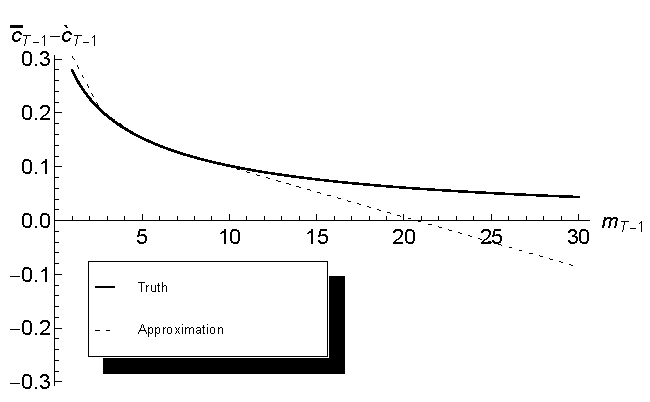
\includegraphics[width=0.8\linewidth]{files/ExtrapProblemPlot-3aca7a9ea92a117508bb3b02a78921ba.pdf}
\caption[]{For Large Enough $\mNrm_{T -1}$, Predicted Precautionary Saving is Negative (Oops!)}
\label{fig:ExtrapProblem}
\end{figure}

This error cannot be fixed by extending the upper gridpoint; in the presence of
serious uncertainty, the consumption rule will need to be evaluated outside of
\textit{any} prespecified grid (because starting from the top gridpoint, a large enough
realization of the uncertain variable will push next period's realization of
assets above that top; a similar argument applies below the bottom gridpoint).
While a judicious extrapolation technique can prevent this problem from being
fatal (for example by carefully excluding negative precautionary saving), the
problem is often dealt with using inelegant methods whose implications for the
accuracy of the solution are difficult to gauge.

\section{The Method of Moderation}

\subsection{The Optimist, the Pessimist, and the Realist}

As a preliminary to our solution, define $\hNrmOpt_{t}$\footnote{In normalized variables, with constant interest factor $\Rfree>1$ and
deterministic permanent growth factor $\PermGroFac$, and setting
$\tranShk_{t+n}=1$ (the optimist's assumption), human wealth can be
calculated in three equivalent ways: (i) finite-horizon backward recursion:
$\hNrmOpt_{T} = 0$, $\hNrmOpt_{t} = (\PermGroFac/\Rfree)\,(1 + \hNrmOpt_{t+1})$
for $t = T -1, T -2, \ldots$; (ii) finite-horizon forward sum:
$\hNrmOpt_{t} = \sum_{n=1}^{T -t}(\PermGroFac/\Rfree)^{n}$; (iii) infinite-horizon
limit: $\hNrmOpt_{\infty} = \PermGroFac/(\Rfree -\PermGroFac)$ provided
$\Rfree>\PermGroFac$. When $\PermGroFac=1$ (as used in the main text),
these expressions simplify to $\hNrmOpt_{t} = \sum_{n=1}^{T -t}(1/\Rfree)^{n}$
and $\hNrmOpt_{\infty} = 1/(\Rfree -1)$.}
as end-of-period human wealth (the present discounted value of future labor
income) for a perfect foresight version of the problem of a `risk optimist:' a
period-$t$ consumer who believes with perfect confidence that the shocks will
always take their expected value of 1,
$\tranShk_{t+n} = \Ex[\tranShk]=1~\forall~n>0$. The solution to a perfect
foresight problem of this kind takes the form\footnote{For a derivation, see \citet{CarrollShanker2024}; $\MPCmin_{t}$ is defined therein as the MPC of the perfect foresight consumer with horizon $T -t$.}

\begin{equation}
\label{eq:cFuncOpt}
\cFuncOpt_{t}(\mNrm_{t}) = (\mNrm_{t} + \hNrmOpt_{t})\MPCmin_{t}
\end{equation}

for a constant minimal marginal propensity to consume $\MPCmin_{t}$ given
below.\footnote{This represents
the MPC of the perfect foresight consumer with horizon $T -t$, corresponding to
the optimist's consumption behavior when market resources are very large.
Equivalent expressions: (i) backward recursion
$\MPCmin_{t}=\MPCmin_{t+1}/\bigl(\MPCmin_{t+1}+\AbsPatFac/\Rfree\bigr)$
with terminal condition $\MPCmin_T=1$; (ii) finite-horizon forward sum
$\MPCmin_{t}=\bigl(\sum_{n=0}^{T -t}(\AbsPatFac/\Rfree)^{n}\bigr)^{ -1}$;
(iii) closed-form infinite-horizon limit $\MPCmin_{\infty}=1 -\AbsPatFac/\Rfree$.} We similarly define
$\hNrmPes_{t}$\footnote{In normalized variables, with constant interest factor $\Rfree>1$ and
deterministic permanent growth factor $\PermGroFac$, and setting
$\tranShk_{t+n}=\tranShkMin~\forall~n>0$ (the pessimist's assumption),
minimal human wealth can be calculated in three equivalent ways.
In the Friedman-Muth process, $\tranShkMin \equiv 0$ since $\WorstProb > 0$
represents the probability of unemployment (zero transitory income).
The three calculation methods are: (i) finite-horizon backward recursion: $\hNrmPes_{T}=0$,
$\hNrmPes_{t}=(\PermGroFac/\Rfree)\,\bigl(\tranShkMin + \hNrmPes_{t+1}\bigr)$
for $t = T -1, T -2, \ldots$; (ii) finite-horizon forward sum:
$\hNrmPes_{t}=\tranShkMin\,\sum_{n=1}^{T -t}(\PermGroFac/\Rfree)^{n}$;
(iii) infinite-horizon limit: $\hNrmPes_{\infty}=\tranShkMin\,\PermGroFac/(\Rfree -\PermGroFac)$
provided $\Rfree>\PermGroFac$. When $\tranShkMin=0$ (unemployment possible),
these expressions reduce to $\hNrmPes_{t}=0$.} as `minimal human wealth,' the present
discounted value of labor income if the shocks were to take on their worst
value in every future period
$\tranShk_{t+n} = 0$ or $\tranShkMin$ $\forall~n>0$ (which we define as corresponding to the beliefs of a `pessimist').

We will call a `realist' the consumer who correctly perceives the true
probabilities of the future risks and optimizes accordingly.

A first useful point is that, for the realist, a lower bound for the level of
market resources is $\mNrmMin_{t} = -\hNrmPes_{t}$ \citep{Aiyagari1994, Huggett1993}, because if $\mNrm_{t}$
equalled this value then there would be a positive finite chance (however small)
of receiving $\tranShk_{t+n} = 0$ or $\tranShkMin$ in every future period, which
would require the consumer to set $\cNrm_{t}$ to zero in order to guarantee that the
intertemporal budget constraint holds. Since consumption of zero yields negative
infinite utility, the solution to the realist consumer's problem is not well
defined for values of $\mNrm_{t} < \mNrmMin_{t}$ \citep{Zeldes1989, Deaton1991}, and the limiting value of the
realist's $\cNrm_{t}$ is zero as $\mNrm_{t} \downarrow \mNrmMin_{t}$.

Given this result, it will be convenient to define `excess' market resources as
the amount by which actual resources exceed the lower bound, and `excess' human
wealth as the amount by which mean expected human wealth exceeds guaranteed
minimum human wealth:

\begin{equation}
\begin{aligned}
\mNrmEx_{t} &= \mNrm_{t}+\overbrace{\hNrmPes_{t}}^{=-\mNrmMin} \\
\hNrmEx_{t} &= \hNrmOpt_{t}-\hNrmPes_{t}.
\end{aligned}
\end{equation}

We can now transparently define the optimal consumption rules for the two
perfect foresight problems, those of the `optimist' and the `pessimist.' The
`pessimist' perceives human wealth to be equal to its minimum feasible value
$\hNrmPes_{t}$ with certainty, so consumption is given by the perfect foresight
solution

\begin{equation}
\begin{aligned}
\cFuncPes_{t}(\mNrm_{t}) &= (\mNrm_{t}+\hNrmPes_{t})\MPCmin_{t} \\
&= \mNrmEx_{t}\MPCmin_{t} .
\end{aligned}
\end{equation}

The `optimist,' on the other hand, pretends that there is no uncertainty about
future income, and therefore consumes

\begin{equation}
\begin{aligned}
\cFuncOpt_{t}(\mNrm_{t}) &= (\mNrm_{t} +\hNrmPes_{t} - \hNrmPes_{t} + \hNrmOpt_{t} )\MPCmin_{t} \\
&= (\mNrmEx_{t} + \hNrmEx_{t})\MPCmin_{t} \\
&= \cFuncPes_{t}(\mNrm_{t})+\hNrmEx_{t} \MPCmin_{t} .
\end{aligned}
\end{equation}

\subsection{The Consumption Function}

It seems obvious that the spending of the realist will be strictly greater than
that of the pessimist and strictly less than that of the optimist.
Figure~\ref{fig:IntExpFOCInvPesReaOptNeedHi} illustrates the proposition for the
consumption rule in period $T -1$.

\begin{figure}[!htbp]
\centering
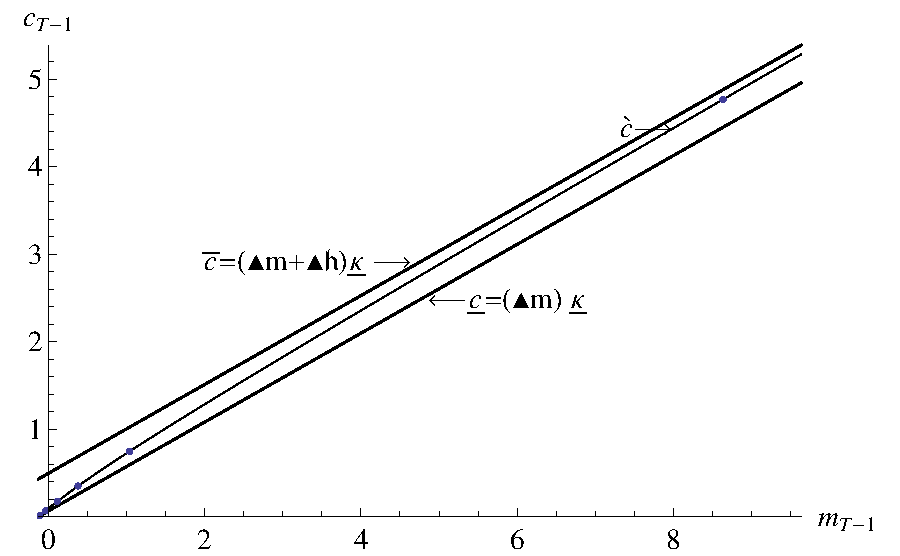
\includegraphics[width=0.8\linewidth]{files/IntExpFOCInvPesReaOp-fb624fab0b4a4099fba4af3d4745d311.pdf}
\caption[]{Moderation Illustrated: $\cFuncPes < \cFuncApprox < \cFuncOpt$}
\label{fig:IntExpFOCInvPesReaOptNeedHi}
\end{figure}

The proof is more difficult than might be imagined, but the necessary work is
done in \citet{CarrollShanker2024}\footnote{Under prudence ($\uFunc''' > 0$) and bounded shocks with strictly positive support
(nondegenerate lower and upper bounds), the consumption function is strictly
increasing and concave, and the moderation ratio lies in $(0,1)$; see \citet{CarrollShanker2024}.} so we will take the proposition as
a fact and proceed by manipulating the inequality:

\begin{equation}
\begin{array}{rcl}
\cFuncOpt_{t}(\mNrmMin_{t}+\mNrmEx_{t}) > & \cFuncReal_{t}(\mNrmMin_{t}+\mNrmEx_{t}) & > \cFuncPes_{t}(\mNrmMin_{t}+\mNrmEx_{t}) \\
-\cFuncOpt_{t}(\mNrmMin_{t}+\mNrmEx_{t}) < & -\cFuncReal_{t}(\mNrmMin_{t}+\mNrmEx_{t}) & < -\mNrmEx_{t} \MPCmin_{t} \\
0 < & \cFuncOpt_{t}(\mNrmMin_{t}+\mNrmEx_{t})-\cFuncReal_{t}(\mNrmMin_{t}+\mNrmEx_{t}) & < \hNrmEx_{t} \MPCmin_{t} \\
0 < & \underbrace{\left(\frac{\cFuncOpt_{t}(\mNrmMin_{t}+\mNrmEx_{t})-\cFuncReal_{t}(\mNrmMin_{t}+\mNrmEx_{t})}{\hNrmEx_{t} \MPCmin_{t}}\right)}_{\equiv \modRte_{t}} & < 1
\end{array}
\end{equation}

where the fraction in the middle of the last inequality is the ratio of actual
precautionary saving (the numerator is the difference between perfect-foresight
consumption and optimal consumption in the presence of uncertainty) to the
maximum conceivable amount of precautionary saving (the amount that would be
undertaken by the pessimist who consumes nothing out of any future income beyond
the perfectly certain component).\footnote{This ratio is strictly between 0 and 1 for all $\mNrm_{t} > \mNrmMin_{t}$ under strict
monotonicity of the consumption function, which is ensured by prudence ($\uFunc''' > 0$)
and bounded shocks \citep{CarrollKimball1996}, as demonstrated in \citet{CarrollShanker2024}. The denominator
$\hNrmEx_{t} \MPCmin_{t}$ is constant in $\mNrm_{t}$ within a given period, so the ratio is
well-defined. Equivalently, precautionary saving satisfies
$\cFuncOpt_{t} -\cFuncReal_{t} = \modRte_{t}\,\hNrmEx_{t} \MPCmin_{t}$ with $\modRte_{t}\in(0,1)$,
which ensures it is strictly positive.} Defining
$\logmNrmEx_{t} = \log \mNrmEx_{t}$ (which can range from $-\infty$ to
$\infty$), the object in the middle of the last inequality is

\begin{equation}
\label{eq:koppa}
\modRte_{t}(\logmNrmEx_{t}) \equiv  \left(\frac{\cFuncOpt_{t}(\mNrmMin_{t}+e^{\logmNrmEx_{t}})-\cFuncReal_{t}(\mNrmMin_{t}+e^{\logmNrmEx_{t}})}{\hNrmEx_{t} \MPCmin_{t}}\right),
\end{equation}

and we now define

\begin{equation}
\label{eq:chi}
\begin{aligned}
\logitModRteFunc_{t}(\logmNrmEx_{t}) &= \log \left(\frac{1-\modRte_{t}(\logmNrmEx_{t})}{\modRte_{t}(\logmNrmEx_{t})}\right) \\
&= \log \left(1/\modRte_{t}(\logmNrmEx_{t})-1\right)
\end{aligned}
\end{equation}

which has the virtue that it is \textit{asymptotically linear} in the limit as
$\logmNrmEx_{t}$ approaches $+\infty$.\footnote{Under prudence ($\uFunc''' > 0$) and GIC, $\logitModRteFunc_{t}(\logmNrmEx_{t})$ is
asymptotically linear: its slope converges to a constant $\alpha_{t} \ge 0$ as $\logmNrmEx_{t} \to +\infty$. At the
infinite limit $\alpha_{t}$ may equal 0; on any finite grid, the boundary slope used
in computation is strictly positive. For practical numerical work on finite grids,
we extrapolate $\logitModRteFunc_{t}$ linearly using that boundary slope. This approach
preserves $\modRte_{t}\in(0,1)$ and hence $\cFuncPes_{t} < \cFuncApprox_{t} < \cFuncOpt_{t}$,
ensuring that precautionary saving $\cFuncOpt_{t} -\cFuncApprox_{t}$ remains strictly
positive over the extrapolation domain.}

Given $\logitModRteFunc$, the consumption function can be recovered from

\begin{equation}
\label{eq:cFuncHi}
\cFuncReal_{t} = \cFuncOpt_{t}-\overbrace{\frac{1}{1+\exp(\logitModRteFunc_{t})}}^{=\modRte_t} \hNrmEx_{t} \MPCmin_{t}.
\end{equation}

Thus, the procedure is to calculate $\logitModRteFunc_{t}$ at the points
$\mathbf{\logmNrmEx}_{t}$ corresponding to the log of the $\mNrmEx_{t}$ points
defined above, and then using these to construct an interpolating approximation
$\logitModRteFuncApprox_{t}$ from which we indirectly obtain our approximated
consumption rule $\cFuncReal_{t}$ by substituting $\logitModRteFuncApprox_{t}$ for
$\logitModRteFunc$ in equation (\ref{eq:cFuncHi}).

Because this method relies upon the fact that the problem is easy to solve if
the decision maker has unreasonable views (either in the optimistic or the
pessimistic direction), and because the correct solution is always between these
immoderate extremes, we call our solution procedure the `method of moderation.'

Results are shown in Figure~\ref{fig:ExtrapProblemSolved}; a reader with very good
eyesight might be able to detect the barest hint of a discrepancy between the
Truth and the Approximation at the far righthand edge of the figure - a stark
contrast with the calamitous divergence evident in Figure~\ref{fig:ExtrapProblem}.

\begin{figure}[!htbp]
\centering
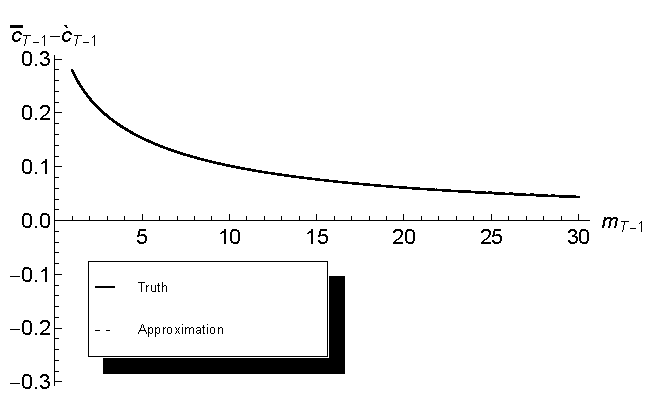
\includegraphics[width=0.8\linewidth]{files/ExtrapProblemSolvedP-056ca09fcb07ee29f643c2a27cdfd6bf.pdf}
\caption[]{Extrapolated $\cFuncApprox_{t -1}$ Constructed Using the Method of Moderation}
\label{fig:ExtrapProblemSolved}
\end{figure}

\subsection{The Value Function}

Often it is useful to know the value function as well as the consumption rule.
Fortunately, many of the tricks used when solving for the consumption rule have
a direct analogue in approximation of the value function.

Consider the perfect foresight (or ``optimist's'') problem in period $T -1$. Using
the fact that in a perfect foresight model the growth factor for consumption is
constant, we can use $\cNrm_{t} = \AbsPatFac \cdot \cNrm_{t -1}$ to calculate the value function in
period $T -1$:

\begin{equation}
\begin{aligned}
\vFuncOpt_{T-1}(\mNrm_{T-1}) &\equiv  \uFunc(\cNrm_{T-1})+\DiscFac \uFunc(\cNrm_{T}) \\
&= \uFunc(\cNrm_{T-1})\left(1+\DiscFac \AbsPatFac^{1-\CRRA}\right) \\
&= \uFunc(\cNrm_{T-1})\left(1+\AbsPatFac/\Rfree\right) \\
&= \uFunc(\cNrm_{T-1})\underbrace{\PDV_{T-1}^{T}(\cNrm)/\cNrm_{T-1}}_{\equiv \PDVCoverc_{T-1}^{T}}
\end{aligned}
\end{equation}

where $\PDVCoverc_{t}^{T}=\PDV_{t}^{T}(\cNrm)/\cNrm_{t}$ is the present discounted value
of consumption, normalized by current consumption. Using the fact demonstrated
in \citet{CarrollShanker2024} that
$\PDVCoverc_{t}^{T}=\MPCmin_{t}^{ -1}$\footnote{Under perfect foresight with time-invariant $\DiscFac$ and $\Rfree$, consumption
grows at the constant gross rate $\AbsPatFac$, so $\cLvl_{t+n}=\cLvl_{t}\,\AbsPatFac^{n}$.
Discounting each term by $\Rfree^{ -n}$ yields the present discounted value ratio:
$(\PDV_{t}^{T}(\cLvl)/\cLvl_{t})=\sum_{n=0}^{T -t}(\AbsPatFac/\Rfree)^{n}$.
Hence $\PDVCoverc_{t}^{T}=\sum_{n=0}^{T -t}(\AbsPatFac/\Rfree)^{n}=\MPCmin_{t}^{ -1}$.
When working with normalized variables, replace $\cLvl$ with $\cNrm$; the identity
remains unchanged.}, a similar function can be
constructed recursively for earlier periods, yielding the general expression

\begin{equation}
\label{eq:vFuncPF}
\begin{aligned}
\vFuncOpt_{t}(\mNrm_{t}) &= \uFunc(\cFuncOpt_{t}(\mNrm_{t}))\PDVCoverc_{t}^{T} \\
&= \uFunc(\cFuncOpt_{t})\MPCmin_{t}^{-1} \\
&= \uFunc((\mNrmEx_{t}+\hNrmEx_{t})\MPCmin_{t}) \MPCmin_{t}^{-1} \\
&= \left[(\mNrmEx_{t}+\hNrmEx_{t})^{1-\CRRA}/(1-\CRRA)\right] \cdot \left[\MPCmin_{t}^{1-\CRRA} \cdot \MPCmin_{t}^{-1}\right] \\
&= \uFunc(\mNrmEx_{t}+\hNrmEx_{t})\MPCmin_{t}^{-\CRRA}.
\end{aligned}
\end{equation}

This can be transformed as

\begin{equation}
\begin{aligned}
\vInvOpt_{t} &\equiv  \left((1-\CRRA)\vFuncOpt_{t}\right)^{1/(1-\CRRA)}   \\
&= \cNrm_{t}(\PDVCoverc_{t}^{T})^{1/(1-\CRRA)} \\
&= (\mNrmEx_{t}+\hNrmEx_{t})\MPCmin_{t}^{-\CRRA/(1-\CRRA)}
\end{aligned}
\end{equation}

We apply the same transformation to the value function for the problem with
uncertainty (the ``realist's'' problem):

\begin{equation}
\vInvReal_{t} = \left((1-\CRRA)\vFuncReal_{t}(\mNrm_{t})\right)^{1/(1-\CRRA)}
\end{equation}

and an excellent approximation to the value function can be obtained by
calculating the values of $\vInvReal$ at the same gridpoints used by the
consumption function approximation, and interpolating among those points.

However, as with the consumption approximation, we can do even better if we
realize that the $\vInvOpt$ function for the optimist's problem is an upper
bound for the $\vInv$ function in the presence of uncertainty, and the value
function for the pessimist is a lower bound. Analogously to (\ref{eq:koppa}),
define an upper-case

\begin{equation}
\label{eq:KoppaUpper}
\valModRteReal_{t}(\logmNrmEx_{t}) = \left(\frac{\vInvOpt_{t}(\mNrmMin_{t}+e^{\logmNrmEx_{t}})-\vInvReal_{t}(\mNrmMin_{t}+e^{\logmNrmEx_{t}})}{\hNrmEx_{t} \MPCmin_{t} (\PDVCoverc_{t}^{T})^{1/(1-\CRRA)}}\right)
\end{equation}

and an upper-case version of the $\logitModRteFunc$ equation in (\ref{eq:chi}):

\begin{equation}
\label{eq:ChiUpper}
\begin{aligned}
\logitValModRteReal_{t}(\logmNrmEx_{t}) &= \log \left(\frac{1-\valModRteReal_{t}(\logmNrmEx_{t})}{\valModRteReal_{t}(\logmNrmEx_{t})}\right) \\
&= \log \left(1/\valModRteReal_{t}(\logmNrmEx_{t})-1\right)
\end{aligned}
\end{equation}

and if we approximate these objects then invert them (as above with the $\modRte$
and $\logitModRteFunc$ functions) we obtain a very high-quality approximation to our
inverted value function at the same points for which we have our approximated
value function:

\begin{equation}
\vInvReal_{t} = \vInvOpt_{t}-\overbrace{\left(\frac{1}{1+\exp(\logitValModRteReal_{t})}\right)}^{=\valModRteReal_{t}} \hNrmEx_{t} \MPCmin_{t} (\PDVCoverc_{t}^{T})^{1/(1-\CRRA) }
\end{equation}

from which we obtain our approximation to the value function as $\vFuncReal_{t} = \uFunc(\vInvReal_{t})$.

\section{Extensions}

\subsection{A Tighter Upper Bound}

\citet{CarrollShanker2024} derives an upper limit
$\MPCmax_{t}$\footnote{This represents
the MPC when market resources approach the natural borrowing constraint, where the
consumer faces maximum uncertainty about future income.     In the
Friedman-Muth process \citep{CarrollToche2009}, $\WorstProb$ is the probability that the transitory shock
equals zero: $\WorstProb = \Pr(\tranShk = 0)$, representing the unemployment probability.
Equivalent expressions: (i) backward recursion
$\MPCmax_{t} = 1 - \WorstProb^{1/\CRRA} \frac{\AbsPatFac}{\Rfree} (1 + \MPCmax_{t+1})$
with terminal condition $\MPCmax_T = 1$; (ii) finite-horizon forward sum
$\MPCmax_{t} = 1 - \WorstProb^{1/\CRRA} \frac{\AbsPatFac}{\Rfree} \sum_{n=0}^{T -t}\left(\WorstProb^{1/\CRRA} \frac{\AbsPatFac}{\Rfree}\right)^{n}$;
(iii) closed-form infinite-horizon limit
$\MPCmax_{\infty} = 1 - \WorstProb^{1/\CRRA} \frac{\AbsPatFac}{\Rfree}$.} for the MPC as $\mNrm_{t}$ approaches its
lower bound, extending the explicit limiting MPC formulas established in buffer-stock theory \citep{MaToda2021SavingRateRich}. Using this fact plus the strict concavity of the consumption
function yields the proposition that

\begin{equation}
\cFuncReal_{t}(\mNrmMin_{t}+\mNrmEx_{t}) < \MPCmax_{t} \mNrmEx_{t}.
\end{equation}

The solution method described above does not guarantee that approximated
consumption will respect this constraint between gridpoints, and a failure to
respect the constraint can occasionally cause computational problems in solving
or simulating the model. Here, we describe a method for constructing an
approximation that always satisfies the constraint.

Defining $\mNrmCusp_{t}$ as the \textit{cusp} point where the two upper bounds intersect
(where $\mNrmCuspEx_{t}\equiv\mNrmCusp_{t} -\mNrmMin_{t}$):

\begin{equation}
\begin{array}{rclcll}
\bigl(\mNrmCuspEx_{t} + \hNrmEx_{t}\bigr)\,\MPCmin_{t} &= & \MPCmax_{t}\,\mNrmCuspEx_{t} & & \\
\mNrmCuspEx_{t} &= & \dfrac{\MPCmin_{t}\,\hNrmEx_{t}}{\MPCmax_{t}-\MPCmin_{t}} & & \\
\mNrmCusp_{t} &= & -\hNrmPes_{t} + \dfrac{\MPCmin_{t}\,\bigl(\hNrmOpt_{t}-\hNrmPes_{t}\bigr)}{\MPCmax_{t}-\MPCmin_{t}},
\end{array}
\end{equation}

we want to construct a consumption function for
$\mNrm_{t} \in (\mNrmMin_{t}, \mNrmCusp_{t}]$ that respects the tighter upper
bound:

\begin{equation}
\begin{array}{rcl}
\mNrmEx_{t} \MPCmin_{t} < & \cFuncReal_{t}(\mNrmMin_{t}+\mNrmEx_{t}) & < \MPCmax_{t} \mNrmEx_{t} \\
\mNrmEx_{t}(\MPCmax_{t}- \MPCmin_{t}) > & \MPCmax_{t} \mNrmEx_{t}-\cFuncReal_{t}(\mNrmMin_{t}+\mNrmEx_{t}) & > 0 \\
1 > & \left(\frac{\MPCmax_{t} \mNrmEx_{t}-\cFuncReal_{t}(\mNrmMin_{t}+\mNrmEx_{t})}{\mNrmEx_{t}(\MPCmax_{t}- \MPCmin_{t})}\right) & > 0.
\end{array}
\end{equation}

Again defining $\logmNrmEx_{t} =\log \mNrmEx_{t}$, the object in the middle of
the inequality is

\begin{equation}
\label{eq:koppaLo}
\modRtePes_{t}(\logmNrmEx_{t}) \equiv  \frac{\MPCmax_{t}-\cFuncReal_{t}(\mNrmMin_{t}+e^{\logmNrmEx_{t}})e^{-\logmNrmEx_{t}}}{\MPCmax_{t}-\MPCmin_{t}}.
\end{equation}

As $\mNrm_{t}$ approaches $-\mNrmMin_{t}$, $\modRtePes_{t}(\logmNrmEx_{t})$
converges to 0, while as $\mNrm_{t}$ approaches $+\infty$,
$\modRtePes_{t}(\logmNrmEx_{t})$ approaches 1.

As before, we can derive an approximated consumption function; call it
$\cFuncLoTightUpBd_{t}$. This function will clearly do a better job approximating
the consumption function for low values of $\mNrm_{t}$ while the previous
approximation will perform better for high values of $\mNrm_{t}$.

For middling values of $\mNrm$ it is not clear which of these functions will
perform better. However, an alternative is available which performs well. Define
the highest gridpoint below $\mNrmCusp_{t}$ as $\mNrmLoTightUpBd$ and the lowest
gridpoint above $\mNrmCusp_{t}$ as $\mNrmHiTightUpBd$. Then there will be a unique
interpolating polynomial that matches the level and slope of the consumption
function at these two points. Call this function $\cFuncMidTightUpBd_{t}(\mNrm)$.

Using indicator functions that are zero everywhere except for specified
intervals,

\begin{equation}
\begin{aligned}
\mathbf{1}_{\text{Lo}}(\mNrm)  &= 1 \text{~if $\mNrm \leq \mNrmLoTightUpBd \phantom{< \mNrm < \mNrmHiTightUpBd \leq \mNrm}$} \\
\mathbf{1}_{\text{Mid}}(\mNrm) &= 1 \text{~if $\phantom{\mNrm \leq}~ \mNrmLoTightUpBd < \mNrm < \mNrmHiTightUpBd \phantom{\leq \mNrm}$} \\
\mathbf{1}_{\text{Hi}}(\mNrm)  &= 1 \text{~if $\phantom{\mNrm \leq ~\mNrmLoTightUpBd < \mNrm <} \mNrmHiTightUpBd \leq \mNrm$}
\end{aligned}
\end{equation}

we can define a well-behaved approximating consumption function

\begin{equation}
\cFuncApprox_{t} = \mathbf{1}_{\text{Lo}} \cFuncLoTightUpBd_{t} + \mathbf{1}_{\text{Mid}} \cFuncMidTightUpBd_{t}+\mathbf{1}_{\text{Hi}} \cFuncHiTightUpBd_{t}.
\end{equation}

This just says that, for each interval, we use the approximation that is most
appropriate. The function is continuous and once-differentiable everywhere, and
is therefore well behaved for computational purposes.

We now construct an upper-bound value function implied for a consumer whose
spending behavior is consistent with the refined upper-bound consumption rule.

For $\mNrm_{t} \geq \mNrmCusp_{t}$, this consumption rule is the same as
before, so the constructed upper-bound value function is also the same. However,
for values $\mNrm_{t} < \mNrmCusp_{t}$ matters are slightly more complicated.

Start with the fact that at the cusp point,

\begin{equation}
\begin{aligned}
\vFuncOpt_{t}(\mNrmCusp_{t}) &= \uFunc(\cFuncOpt_{t}(\mNrmCusp_{t}))\PDVCoverc_{t}^{T} \\
&=  \uFunc(\mNrmCuspEx_{t} \MPCmax_{t})\PDVCoverc_{t}^{T} .
\end{aligned}
\end{equation}

But for \textit{all} $\mNrm_{t}$,

\begin{equation}
\vFuncOpt_{t}(\mNrm_{t}) = \uFunc(\cFuncOpt_{t}(\mNrm_{t}))+ \wFuncCont(\mNrm_{t}-\cFuncOpt_{t}(\mNrm_{t})),
\end{equation}

and we assume that for the consumer below the cusp point consumption is given by
$\MPCmax_{t} \mNrmEx_{t}$ so for $\mNrm_{t}< \mNrmCusp_{t}$

\begin{equation}
\vFuncOpt_{t}(\mNrm_{t}) = \uFunc( \MPCmax_{t} \mNrmEx_{t})+ \wFuncCont((1-\MPCmax_{t})\mNrmEx_{t}),
\end{equation}

which is easy to compute because
$\wFuncCont(\aNrm_{t}) = \DiscFac \vFuncOpt_{t+1}(\aNrm_{t}\RNrmByG_{t+1}+1)$ where
$\vFuncOpt_{t}$ is as defined above because a consumer who ends the current
period with assets exceeding the lower bound will not expect to be constrained
next period. (Recall again that we are merely constructing an object that is
guaranteed to be an \textit{upper bound} for the value that the `realist' consumer will
experience.) At the gridpoints defined by the solution of the consumption
problem can then construct

\begin{equation}
\vInvOpt_{t}(\mNrm) = ((1-\CRRA)\vFuncOpt_{t}(\mNrm))^{1/(1-\CRRA)}
\end{equation}

which yields the appropriate vector for constructing $\logitValModRteApprox$ and
$\valModRteApprox$. The rest of the procedure is analogous to that performed for the
consumption rule and is thus omitted for brevity.

\begin{figure}[!htbp]
\centering
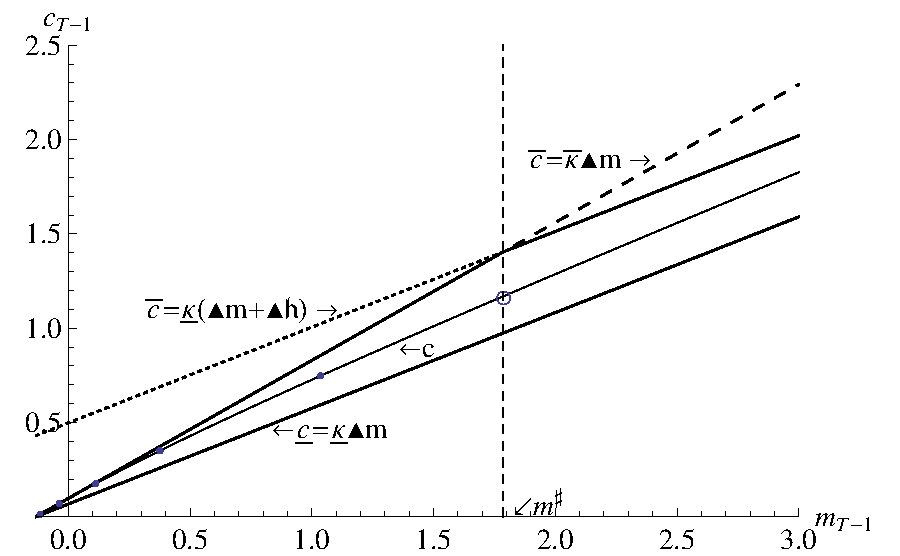
\includegraphics[width=0.8\linewidth]{files/IntExpFOCInvPesReaOp-7e53934f52256b9d0a62f67919fb1d97.pdf}
\caption[]{A Tighter Upper Bound}
\label{fig:IntExpFOCInvPesReaOptNeed45}
\end{figure}

\subsection{Hermite Interpolation}

The numerical accuracy of the method of moderation depends critically on the quality of function approximation between gridpoints \citep{Santos2000}. Our bracketing approach complements work that bounds numerical errors in dynamic economic models \citep{JuddMaliarMaliar2017}. Although linear interpolation that matches the level of $\cFuncReal$ at the gridpoints is simple, Hermite interpolation \citep{Fritsch1980, FritschButland1984, Hyman1983} offers a considerable advantage. By matching both the level and the derivative of the $\cFuncReal_{t}$ function at the gridpoints, the consumption rule derived from such interpolation numerically satisfies the Euler equation at each gridpoint for which the problem has been solved \citep{BenvenisteScheinkman1979, MilgromSegal2002}.

The theoretical foundation for this approach rests on the moderation ratio $\modRte$. This ratio captures how far the realist's consumption lies between the perfect-foresight upper bound and the pessimistic lower bound. Since its log-gap argument $\logmNrmEx$ moves with cash-on-hand relative to human wealth, the derivative measures how quickly the realist closes this gap as available resources shift:

\begin{equation}
\label{eq:modRteMu}
\modRteMu_{t} = \frac{\mNrmEx_{t} (\MPCmin_{t} - \partial \cFuncReal/\partial \mNrm_{t})}{\MPCmin_{t} \hNrmEx_{t}}.
\end{equation}

For numerical stability and interpretation on an unbounded scale, we apply the transformation defined in (\ref{eq:chi}) to the moderation ratio. The derivative of this transformation is:

\begin{equation}
\label{eq:logitModRteMu}
\logitModRteMu_{t} = \frac{\modRteMu_{t}}{(\modRte_{t} - 1) \modRte_{t}}.
\end{equation}

This expression provides the slope data required for cubic Hermite interpolation.\footnote{For cubic Hermite interpolation of the transformed moderation ratio, use node values from the transformation and node slopes $\logitModRteMu$. For improved shape preservation, a monotone cubic Hermite scheme \citep{deBoor2001} can be used, where theoretical slopes serve as targets that may be adjusted to enforce monotonicity.} To recover the realist consumption function from the interpolated transformation, we use the relationship established in (\ref{eq:cFuncHi}). To recover the realist marginal propensity to consume, we differentiate with respect to the transformation:

\begin{equation}
\label{eq:MPCRecovery}
\frac{\partial \cFuncReal_{t}}{\partial \mNrm_{t}} = \MPCmin_{t} \left(1 - \frac{\hNrmEx_{t}}{\mNrmEx_{t}} \logitModRteMu_{t}\right).
\end{equation}

Since we have $\logitModRteMu_{t}$ from the Hermite interpolation, we can compute the realist MPC directly from the interpolated transformation derivatives. This expression reveals that the realist MPC is moderated away from $\MPCmin_{t}$ by the transformation derivative, weighted by the ratio of human wealth to excess market resources. When uncertainty is low, the transformation derivative approaches zero and the realist MPC approaches the optimistic benchmark. Results showing identical MPCs under certain conditions \citep{CKW2021Aggregation} help explain why simple linear bounds work so well in many cases.

We can apply analogous techniques to the value function. Under perfect foresight, consumption grows at a constant rate, making $\PDVCoverc_{t}^{T}$ constant. This implies that the inverse value function for the optimist has a constant slope with respect to cash-on-hand:

\begin{equation}
\label{eq:vInvOptDeriv}
\begin{aligned}
\vInvOptDeriv_{t} &= (\PDVCoverc_{t}^{T})^{1/(1-\CRRA)} \MPCmin_{t} \\
&= \MPCmin_{t}^{-\CRRA/(1-\CRRA)}.
\end{aligned}
\end{equation}

The result in (\ref{eq:vInvOptDeriv}) has important implications for the structure of the value function.\footnote{This confirms that $\vInvOpt_{t}$ is linear in $\mNrm$ and highlights the role of $\MPCmin_{t}$ in scaling marginal utility in the perfect-foresight benchmark. The linearity property simplifies both theoretical analysis and numerical implementation.}

Consider the value analogue of the moderation ratio, which compares the realist's value to the optimist's. The derivative of this ratio with respect to the log-gap argument is:

\begin{equation}
\label{eq:valModRteRealDerivmu}
\valModRteRealDerivmu_{t} = \frac{\mNrmEx_{t} (\vInvOptDeriv_{t} - \vInvRealDeriv_{t})}{\hNrmEx_{t} \vInvOptDeriv_{t}}
\end{equation}

where $\vInvOptDeriv_{t} = \MPCmin_{t}^{ -\CRRA/(1 -\CRRA)}$ from (\ref{eq:vInvOptDeriv}) and $\vInvRealDeriv_{t}$ is the derivative of the realist's inverse value function.

Applying the same transformation to the value-based moderation ratio converts the bounded ratio into an unconstrained slope:

\begin{equation}
\label{eq:logitValModRteRealDerivmu}
\logitValModRteRealDerivmu_{t} = \frac{-\valModRteRealDerivmu_{t}}{\valModRteReal_{t}(1-\valModRteReal_{t})}.
\end{equation}

Since $\vInvReal$ and $\vFuncReal$ are functional inverses, their derivatives are linked by chain-rule relationships. The first derivative is:

\begin{equation}
\label{eq:vInvRealDeriv}
\vInvRealDeriv_{t} = \left( (1-\CRRA) \vFuncReal_{t}(\mNrm_{t})\right)^{-1+1/(1-\CRRA)}  \vFuncRealDeriv_{t}(\mNrm_{t}).
\end{equation}

The first- and second-derivative connections are:

\begin{equation}
\label{eq:vFuncRealDerivatives}
\begin{aligned}
\vFuncRealDeriv_{t} &= \uPrime(\vInvReal_{t}) \, \vInvRealDeriv_{t} \\
\vFuncRealDerivSecond_{t} &= \uDoublePrime(\vInvReal_{t}) \, (\vInvRealDeriv_{t})^2 + \uPrime(\vInvReal_{t}) \, \vInvRealDerivSecond_{t}.
\end{aligned}
\end{equation}

Moreover, if we use the double-derivative calculated in (\ref{eq:vFuncRealDerivatives}) to produce a higher-order Hermite polynomial, our approximation will also match the marginal propensity to consume at the gridpoints.\footnote{This would guarantee that the consumption function generated from the value function would match both the level of consumption and the marginal propensity to consume at the gridpoints, making the numerical differences between the newly constructed consumption function and the highly accurate one constructed earlier negligible within the grid.}

These results provide the theoretical foundation for constructing high-quality cubic Hermite interpolants that preserve both the economic structure and numerical accuracy of the model between gridpoints.

\subsection{Stochastic Rate of Return}

Thus far we have assumed that the interest factor is constant at $\Rfree$.
Extending the previous derivations to allow for a perfectly forecastable
time-varying interest factor $\Risky_{t}$ would be trivial. Allowing for a
stochastic interest factor is less trivial.

The easiest case is where the interest factor is i.i.d.,

\begin{equation}
\label{eq:distRisky}
\log \Risky_{t+n} \sim \Nrml(r + \pi - \std^{2}_{\risky}/2,\std^{2}_{\risky}) ~\forall~n>0
\end{equation}

because in this case \citet{Samuelson1969, Merton1969, Merton1971}
showed that for a consumer without labor income (or with perfectly forecastable
labor income) the consumption function is linear, with an MPC.\footnote{The Merton-Samuelson rule (for iid returns and no labor income, or perfectly forecastable income)
implies a linear consumption function $\cFunc(\mNrm) = \MPC\,\mNrm$, where $\MPC$ is given by
Eq. (\ref{eq:MPCExact}). This result extends naturally to our framework by substituting the
stochastic-return MPC for the perfect foresight MPC. At high wealth, the consumption function becomes asymptotically linear as the precautionary motive vanishes \citep{BBZ2016SkewedWealth}. See \citet{CRRA-RateRisk} for a detailed derivation.}

\begin{equation}
\label{eq:MPCExact}
\MPC_{t} = 1- \left(\DiscFac  \Ex_{t}[\Risky_{t+1}^{1-\CRRA}]\right)^{1/\CRRA}
\end{equation}

and in this case the previous analysis applies once we substitute this MPC for
the one that characterizes the perfect foresight problem without rate-of-return
risk. The more realistic case where the interest factor has some serial
correlation is more complex, and thus left for future work.

In principle, this refinement should be combined with the previous one; further
exposition of this combination is omitted here because no new insights spring
from the combination of the two techniques.

\section{Conclusion}

The method proposed here is not universally applicable. For example, the method
cannot be used for problems for which upper and lower bounds to the `true'
solution are not known. But many problems do have obvious upper and lower
bounds, and in those cases (as in the consumption example used in the paper),
the method may result in substantial improvements in accuracy and stability of
solutions.



%%%%%%%%%%%%%%   Bibliography   %%%%%%%%%%%%%%
\bibliography{main.bib}

\end{document}
